\subsection{Helligkeitsplots}
\label{sec:plots}
\twocolumn[]
      
      \newpage
      \begin{figure}
        \centering
        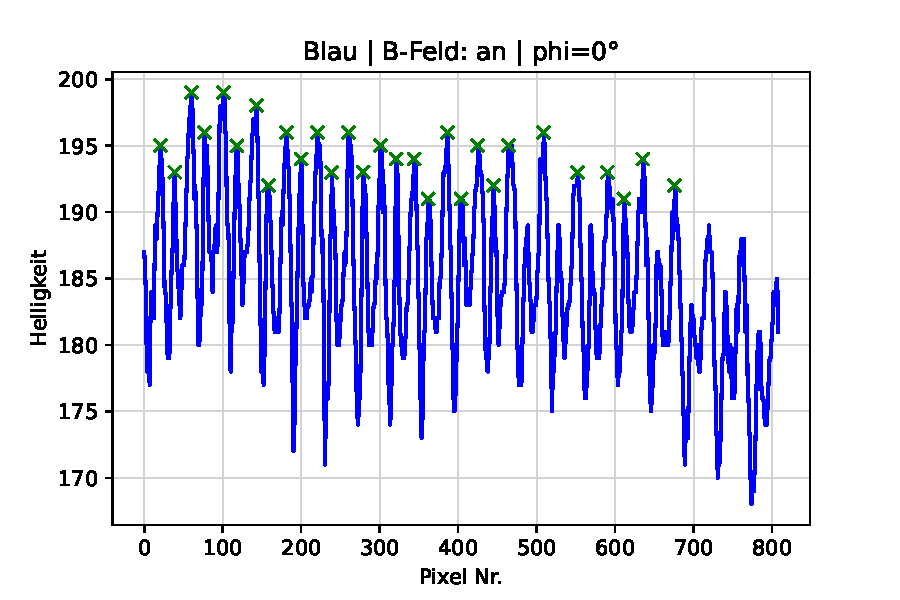
\includegraphics[width=0.5\textwidth]{content/grafiken/blau mit magnet 0 gimbplot.pdf}
        \caption{}
        \label{fig:bmm0}
      \end{figure}
      
      \begin{figure}
        \centering
        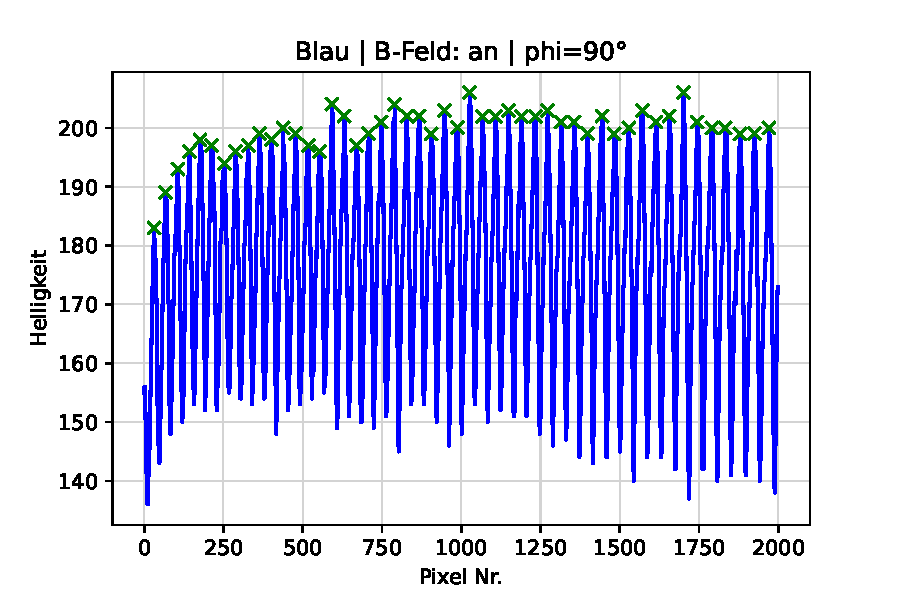
\includegraphics[width=0.5\textwidth]{content/grafiken/blau mit magnet 90 gimbplot.pdf}
        \caption{}
        \label{fig:bmm90}
      \end{figure}
      
      \begin{figure}
        \centering
        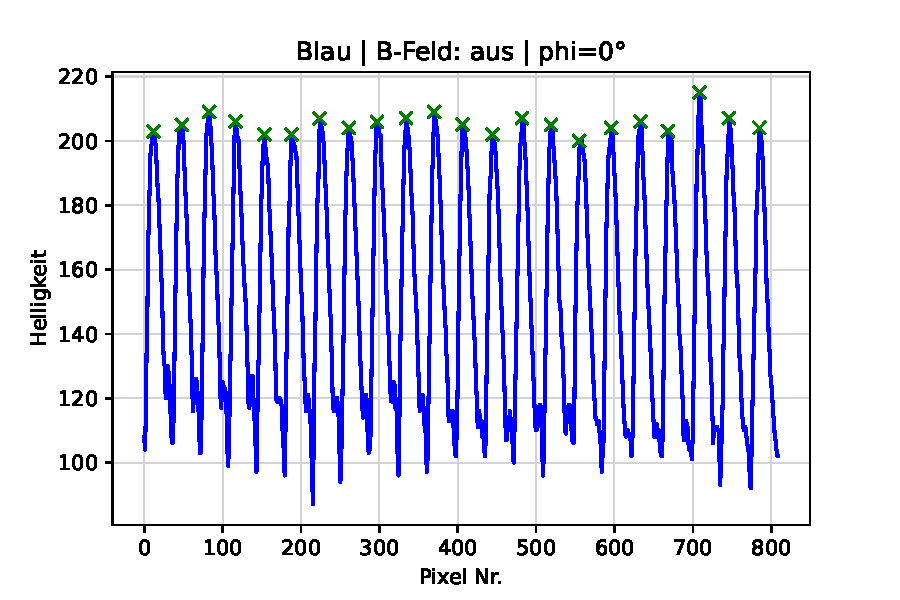
\includegraphics[width=0.5\textwidth]{content/grafiken/blau ohne magnet 0 gimbplot.pdf}
        \caption{}
        \label{fig:bom0}
      \end{figure}
      
      \begin{figure}
        \centering
        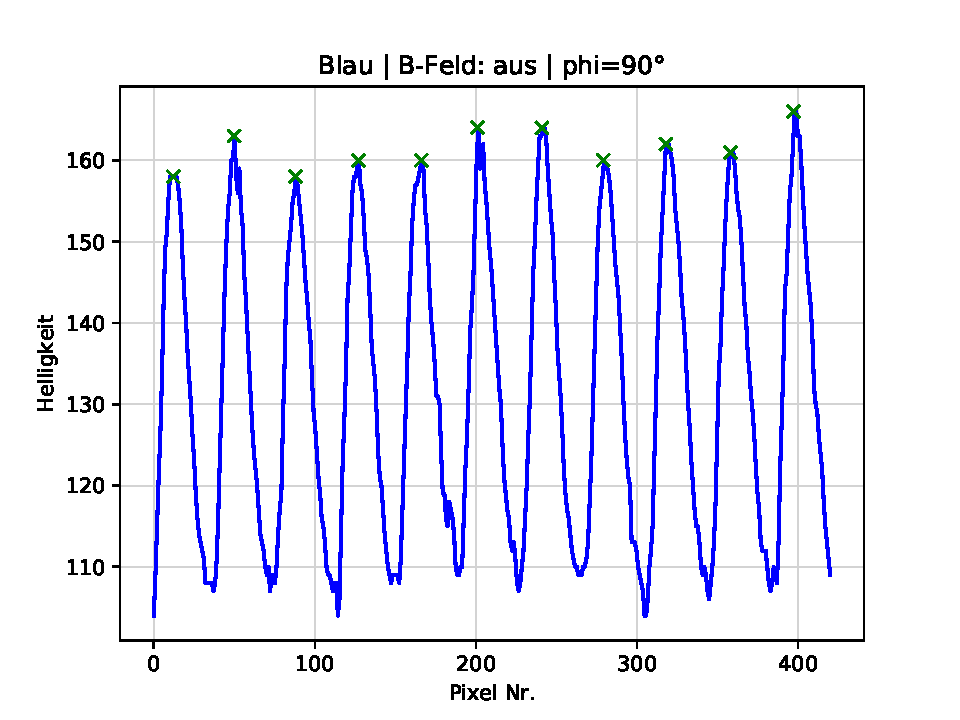
\includegraphics[width=0.5\textwidth]{content/grafiken/blau ohne magnet 90 gimbplot.pdf}
        \caption{}
        \label{fig:bom90}
      \end{figure}
      
      \begin{figure}
        \centering
        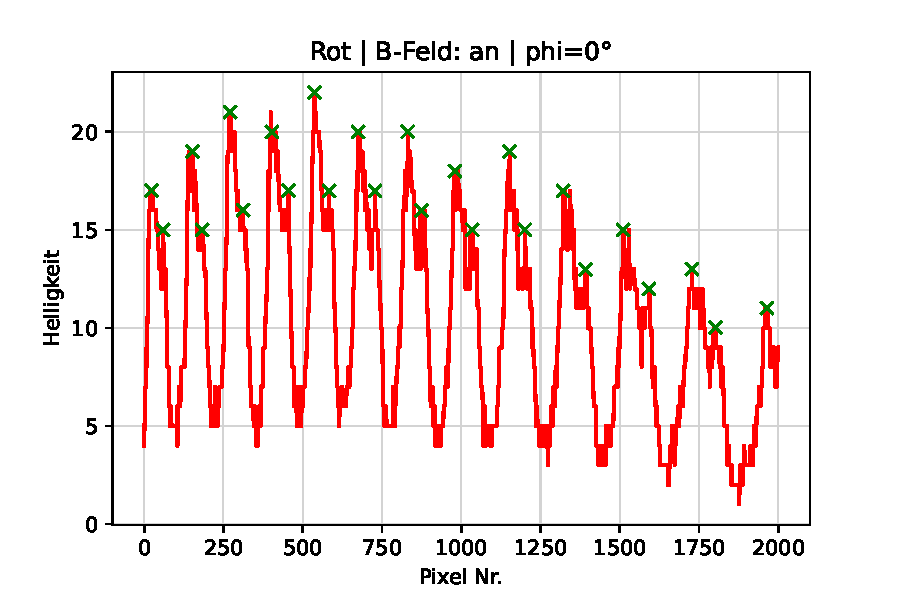
\includegraphics[width=0.5\textwidth]{content/grafiken/rot mit magnet 0 gimbplot.pdf}
        \caption{}
        \label{fig:rmm0}
      \end{figure}
      
      \begin{figure}
        \centering
        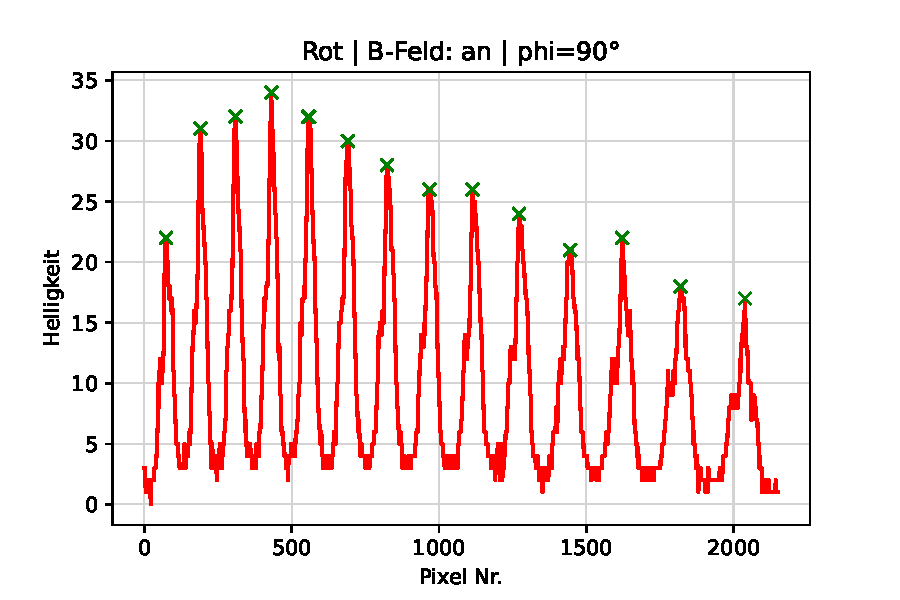
\includegraphics[width=0.5\textwidth]{content/grafiken/rot mit magnet 90 gimbplot.pdf}
        \caption{}
        \label{fig:rmm90}
      \end{figure}
      
      \begin{figure}
        \centering
        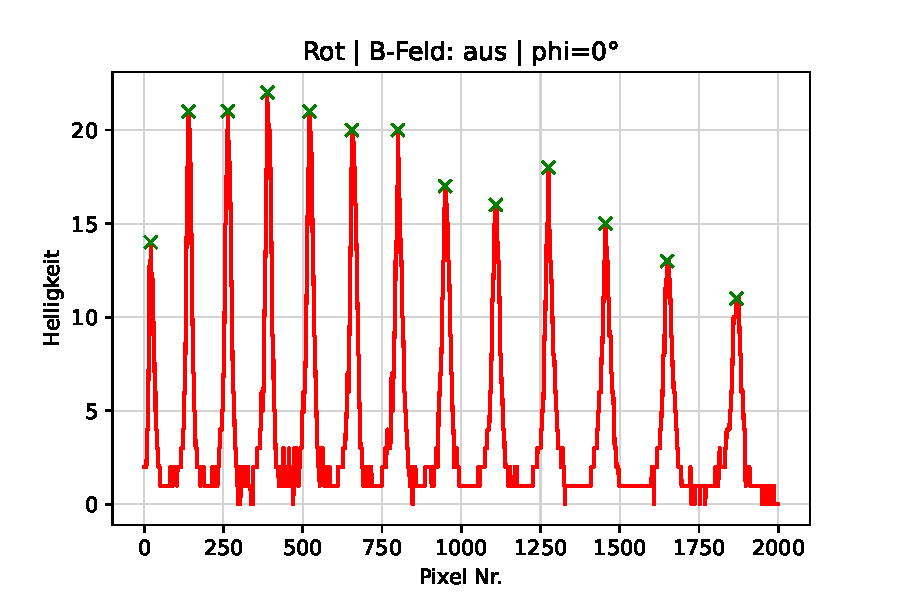
\includegraphics[width=0.5\textwidth]{content/grafiken/rot ohne magnet 0 gimbplot.pdf}
        \caption{}
        \label{fig:rom0}
      \end{figure}
      
      \begin{figure}
        \centering
        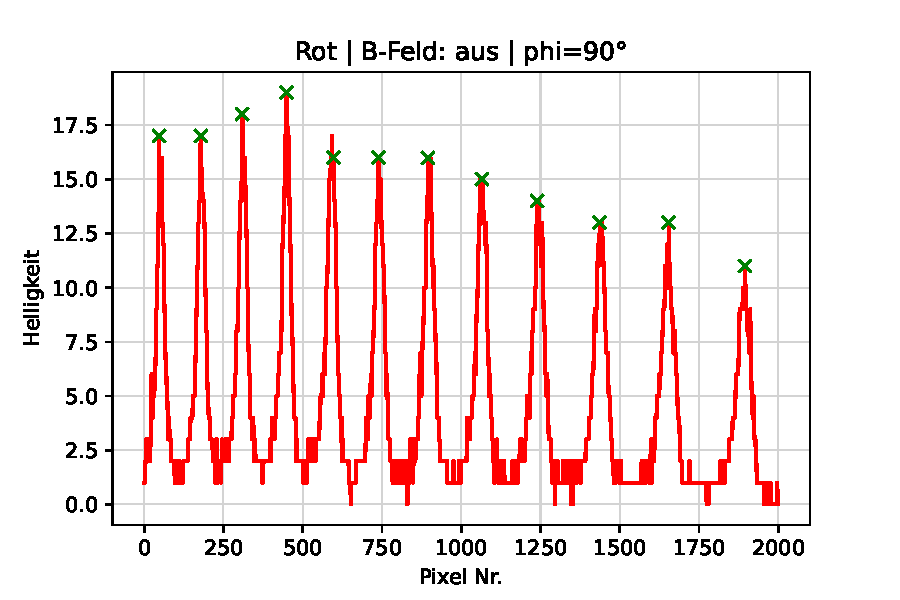
\includegraphics[width=0.5\textwidth]{content/grafiken/rot ohne magnet 90 gimbplot.pdf}
        \caption{}
        \label{fig:rom90}
      \end{figure}
\onecolumn